% !TEX root = ../main.tex
\section{Background} \label{sec::background}
% NOTE: Consider giving PCs the possibility of learning feats from other background, with the restriction that it needs one additional FP. This plays into the dynamism in Yuadrem.
Due to the open-endedness of characters in Yuadrem (see page \pageref{sec::classlessdnd} for more details), small changes are applied to the backgrounds in the official books.
Apart from providing a set of competences, equipment and an initial unique trait, each background has set of associated feats that can be learned at higher levels.

To choose religions and learned languages, refer to their respective sections in pages \pageref{ssec::religions} and \pageref{ssec::languages}.
These are not complete lists by any means, but rather the most common in the civilized world.
You are welcome to talk with your DM about including religions and languages as they may seem fit in your campaign.

For personality traits, ideals, bonds, and flaws, check the official books.

\subsection*{Acolyte} \label{ssec::acolyte}
    Clerics, cultists, fanatics, and priests all share a devotion to something larger to themselves.
    You have spent your life in the service of a temple to a specific god or pantheon of gods.
    You act as an intermediary between the realm of the holy and the mortal world, performing sacred rites and offering sacrifices in order to conduct worshipers into the presence of the divine.

    Choose a god, a pantheon of gods, or some other divine being, and work with your DM to detail the nature of your religious service.
    This god or pantheon may be from any religion as detailed in the religion section (see pages \pageref{ssec::therism} for Therism and \pageref{ssec::religions} for other common religions), or a deity from outside of these pantheons that works with your DM.

    Were you a lesser functionary in a temple, raised from childhood to assist the priests in the sacred rites?
    Or were you a high priest who suddenly experienced a call to serve your god in a different way?
    Perhaps you were the leader of a small cult outside of any established temple structure, or even an occult group that served a fiendish master that you now deny.

    Acolytes are shaped by their experience in temples or other religious communities.
    Their study of the history and tenets of their faith and their relationships to temples, shrines, or hierarchies affect their mannerisms and ideals.

    \subparagraph{Competences} Religion, plus your choice of two from among History, Performance, Persuasion, and a language of your choice.

    \subparagraph{Equipment} A holy symbol representative of your religion, a prayer book or prayer wheel, vestments associated with your role, and a set of common clothes.

    \subsubsection{Voice of your God} \label{feat::voiceofyourgod}
        You are capable of performing any religious ceremony associated to your deity.
        You can do this in any established temple, improvised altar, or public plaza, and can expect to at least gather the attention of those around you.

        If you spend at least an hour performing this activity, you can choose to roll a Charisma (Performance) check contested against a target's --- or targets' --- Wisdom (Insight).
        On a success, they are charmed by you for 1d4 hours.
        This charm ends if you or one of your companions harms the creature.

        Additionally, you might receive a small donation for your performance at the DM's discretion.

    \subsection*{Acolyte Feats}
        \begin{DndTable}[width=\linewidth, header=Acolyte Feats]{ll}
            Acolyte & \textbf{Divine Healing} (page \pageref{feat::divinehealing})                 \\
            Acolyte & \textbf{Divine Inspiration} (page \pageref{feat::divineinspiration})         \\
            Acolyte & \textbf{Guidance} (page \pageref{feat::guidance})                            \\
            Acolyte & \textbf{Incite Respect} (page \pageref{feat::inciterespect})                 \\
            Acolyte & \textbf{Inspiring Leader} (page \pageref{feat::inspiringleader})             \\
            Acolyte & \textbf{Shelter of the Faithful} (page \pageref{feat::shelterofthefaithful})
        \end{DndTable}

        \subsubsection{Divine Healing (2 FP)} \label{feat::divinehealing}
            When you roll a 1 or 2 on a die related to healing or giving temporary hit points to one or more creatures, you can reroll the die and must use the new roll, even if the new is a 1 or a 2.
            Additionally, whenever you heal a creature (including yourself) you heal yourself by 1.
            \paragraph{Requirements} Acolyte background.
        \subsubsection{Divine Inspiration} \label{feat::divineinspiration}
            As an action, you can touch your holy symbol, utter a prayer, and regain one expended spell slot, the level of which can be no higher than 1/5th your level, rounded up.
            You can use this feat once per short rest.
            \paragraph{Requirements} Acolyte background.
        \subsubsection{Guidance} \label{feat::guidance}
            As an action, you give words of encouragement to one willing creature.
            Once during the next minute, the target can roll a d4 and add the number rolled to one ability check of its choice.
            It can roll the die before or after making the ability check.

            Only one creature can be affected by this ability at a time.
            \paragraph{Requirements} Acolyte background
        \subsubsection{Incite Respect} \label{feat::inciterespect}
            Using two actions, you present your holy symbol, and each creature of your choice that can see or hear you within 6 meters of you must succeed on a Wisdom saving throw of DC 12 or be charmed by you until the end of your next turn or until the charmed creature takes any damage.
            You can also cause any of the charmed creatures to drop what they are holding when they fail the saving throw.

            You can use this ability a number of times per short rest equal to your Wisdom modifier (Minimum of one).

            You can learn this feat a total of three times, increasing the DC to 15 the second time and to 18 the third.
            \paragraph{Requirements} Acolyte background
        \subsubsection{Inpiring Leader} \label{feat::inspiringleader}
            You can spend 10 minutes inspiring your companions, shoring up their resolve to fight.
            When you do so, choose up to six friendly creatures (which can include yourself) within 6 meters of you who can see or hear you and who can understand you.
            Each creature can gain temporary hit points equal to your level + your Charisma modifier.
            A creature can't gain temporary hit points from this feat again until it has finished a short rest.
            \paragraph{Requirements} Acolyte or Soldier background.
        \subsubsection{Shelter of the Faithful} \label{feat::shelterofthefaithful}
            Your piety inspires the respect of those who share your faith.
            After performing a religious ceremony of your deity, you and your companions can expect to receive free healing and care at a temple, shrine, or other established presence of your faith, though you must provide any material components needed for spells.
            Those who share your religion will support you (but only you) at a modest lifestyle.

            Additionally, your devotion might rouse members from other religions to look kindly to you.
            After performing a religious ceremony or act of kindness, you can roll an Intelligence (Religion) check contested by the creature's Intelligence (Religion).
            On a success, you gain the benefits from this feat from the creature's creed.
            This check is made with advantage if yours and the target deity share tide, and automatically fails if they are enemy deities from the same pantheon.

            % You might also have ties to a specific temple dedicated to your chosen deity or pantheon, and you have a residence there.
            % This could be the temple where you used to serve, if you remain on good terms with it, or a temple where you have found a new home.
            % While near your temple, you can call upon the priests for assistance, provided the assistance you ask for is not hazardous and you remain in good standing with your temple.
            \paragraph{Requirements} Acolyte background.
\subsection*{Artisan} \label{ssec::artisan}
    Crafters, guild artisans, inventors, and engineers all fall into this category.
    Either as part of a guild or a working solo, you are skilled in a particular field and are closely associated with other artisans.
    You are a well-established part of the mercantile world, freed by talent and wealth from the constraints of a feudal social order.
    You learned your skills as an apprentice to a master artisan, maybe under the sponsorship of a guild, until you became a master in your own right.

    \subparagraph{Competences} A set of artisan's tools of your choice, plus your choice of two from among Insight, Perception, Sleight of Hand, and another set of artisan's tools.

    \subparagraph{Equipment} A set of artisan's tools with which you are proficient, a maker's mark chisel used to mark your handiwork with the symbol of your guild, and a set of traveler's clothes.

    \subsubsection{Cunning Artisan} \label{feat::cunningartisan}
        As part of a short rest, you can harvest materials from the wilds, the city, or a slain beast of size small or larger to create one of the following items: a shield, a club, a javelin, or 1d4 darts or blowgun needles.
        To use this trait, you need a blade, such as a dagger.%, or appropiate artisan's tools, such as leatherworker's tools.

    \subsection*{Artisan Feats}
        \begin{DndTable}[width=\linewidth, header=Artisan Feats]{ll}
            Artisan & \textbf{Artificer's Infusions} (page \pageref{feat::artificersinfusion})         \\
            Artisan & \textbf{Beyond Mastery} (page \pageref{feat::beyondmastery})                     \\
            Artisan & \textbf{Flash of Genius} (page \pageref{feat::flashofgenius})                    \\
            Artisan & \textbf{Guild Membership} (page \pageref{feat::guildmembership})                 \\
            Artisan & \textbf{Known Crafter} (page \pageref{feat::knowncrafter})                       \\
            Artisan & \textbf{Improvised Tools} (page \pageref{feat::improvisedtools})
        \end{DndTable}

        \subsubsection{Artificer's Infusion} \label{feat::artificersinfusion}
            You gain the ability to imbue mundane items with infusions.

            When you gain this feature, pick four infusions to learn, choosing from the Infusions list in page \pageref{ssec::infusions}.
            The description of each of the following infusions details the type of item that can receive it, along with wether the resulting magic item requires attunement.
            Unless an infusion's description says otherwise, you can't learn an infusion more than once.

            Whenever you finish a long rest, you can touch a nonmagical object and imbue it with one of your artificer infusions.
            An infusion works on only certain kinds of objects, as specified in the infusion's description.
            If the item requires attunement, you can attune yourself to it the instant you infuse the item.
            If you decide to attune to the item later, you must do so using the normal process for attunement (see ``Attunement'' in chapter 7 of the Dungeon Master's Guide).

            Your infusion remains in an item indefinitely, but only one object can be infused at a time.
            If you try to exceed your maximum number of infusions, the oldest infusion immediately ends, and then the new infusion applies.

            You can learn this feat 3 times.
            The second and third time, you learn an additional infusion, and increase the number of objects that can be infused at the same time by one.

            \paragraph{Requirements} Artisan background or Skilled proficiency with tinker's tools.
        \subsubsection{Beyond Mastery (2 FP)} \label{feat::beyondmastery}
            Practicing for your whole life, you can take your skill as an artisan further than most mortals.
            You increase your proficiency with a set of artisan's tools from Expert to Legendary, increasing your proficiency bonus to +12.
            \paragraph{Requirements} Artisan background, Expert proficiency with a set of artisan's tools.
        \subsubsection{Flash of Genius} \label{feat::flashofgenius}
            You gain the ability to come up with solutions under pressure.
            When you or another creature you can see within 6 meters of you makes an ability check or a saving throw, you can use an action or your reaction to add your Intelligence modifier to the roll.

            You can use this feature a number of times equal to your Intelligence modifier (minimum of once).
            You regain all expended uses when you finish a short rest.
            \paragraph{Requirements} Artisan or Scholar background.
        \subsubsection{Guild Membership} \label{feat::guildmembership}
            As an known figure of your trade, you can become a member of a guild associated to it.
            This membership provides you with certain benefits.
            Your fellow guild members will provide you with lodging and food if necessary, and pay for your funeral if needed.
            In some cities and towns, a guildhall offers a central place to meet other members of your profession, which can be a good place to meet potential patrons, allies, or hirelings.

            Guilds often wield tremendous political power.
            If you are accused of a crime, your guild will support you if a good case can be made for your innocence or the crime is justifiable.
            You can also gain access to powerful political figures through the guild, if you are a member in good standing.
            Such connections might require the donation to the guild's coffers.

            To maintain your membership, you must pay dues of 5 agnomas per month to the guild.
            If you miss payments, you must make up back dues to remain in the guild's good graces.
            \paragraph{Requirements} Artisan or Merchant background.
        \subsubsection{Known Crafter} \label{feat::knowncrafter}
            Knowing the local trade like the back of your hand, you know where to find the best ingredients for the cheapest prices in a settlement in which you are familiar.
            You can buy components and ingredients related to your craft for half their normal price, and you can tell the quality of a raw material just by looking at it.
            To use this feat you must first gain familiarity with a settlement as part of a long rest.
            \paragraph{Requirements} Artisan background.
        \subsubsection{Improvised Tools} \label{feat::improvisedtools}
            In times of need, your vast experience allows you to improvise solutions, adapt to any adversity, and overcome insurmountable challenges.
            You learn how to produce exactly the tool you need.
            By gathering resources from any environment, you can create one set of artisan's tools with which you are already competent with.
            This creation requires 1 hour of uninterrupted work, which can coincide with a short or long rest.
            Tools conjured via this feat are flimsy at best, and no reasonable person would buy them.
            \paragraph{Requirements} Artisan background.

\thispagestyle{empty}
\begin{tikzpicture}[remember picture,overlay]
    \node[anchor=south east, xshift=0.10cm, yshift=-0.10cm] at (current page.south east) {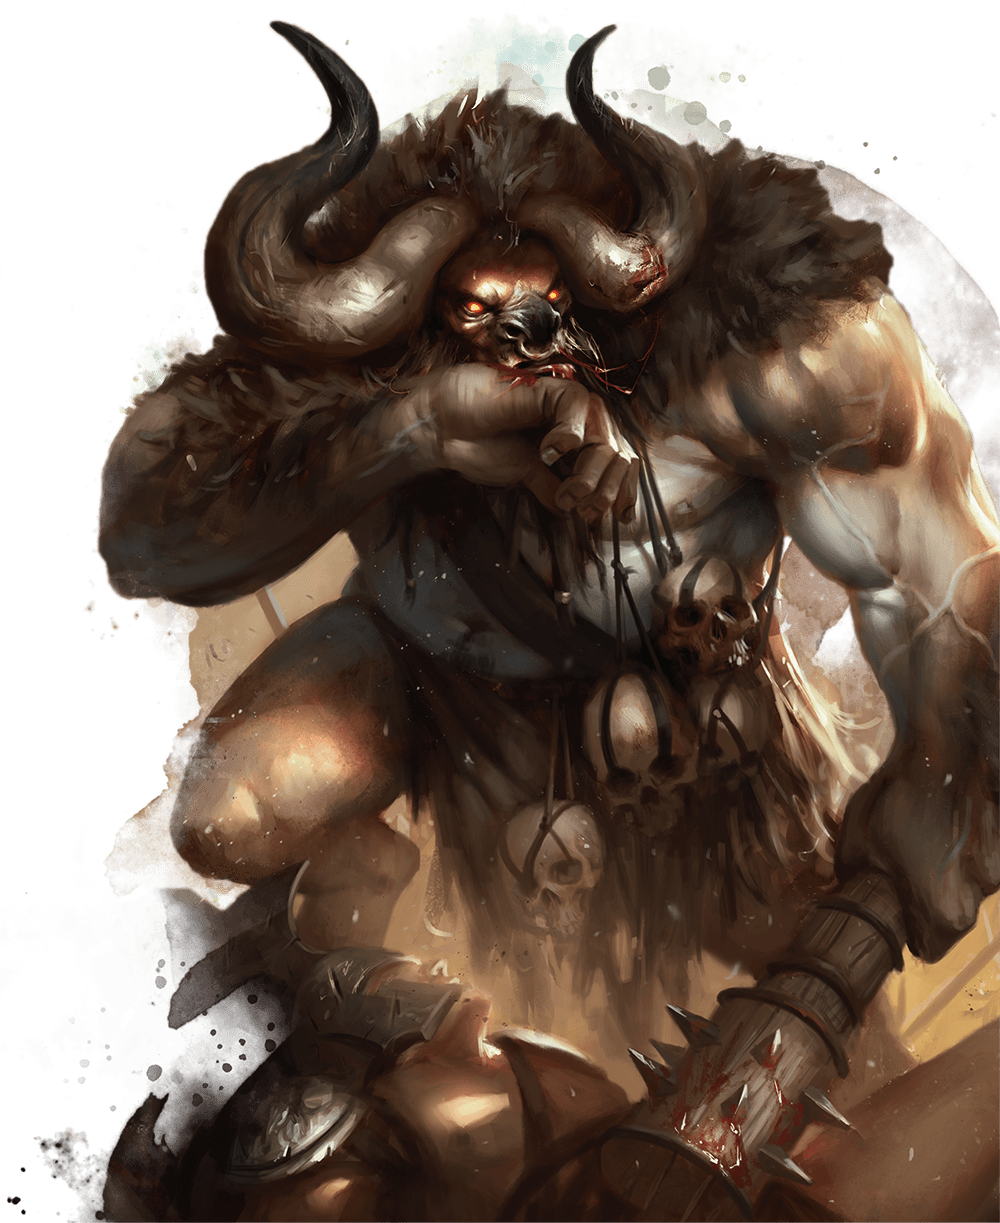
\includegraphics[width=0.50\pdfpagewidth]{05background/img/20treb_gat}};
\end{tikzpicture}

\subsection*{Criminal} \label{ssec::criminal}
    Bandits, pirates, spies, and thieves all share a penchant for crime.
    You are an experienced criminal with a history of breaking the law.
    You have spent a lot of time among other criminals and still have contacts within the criminal underworld.
    You're far closer than most people to the world of murder, theft, and violence that pervades the underbelly of civilization, and you have survived up to this point by flouting the rules and regulations of society.

    There are many kinds of criminals, and within a thieves' guild or similar criminal organization, individual members have particular specialties.
    Even criminals who operate outside of such organizations have strong preferences for certain kinds of crimes over others.
    Choose the role you played in your criminal life.

    \subparagraph{Competences} Deception, plus your choice of two from among Intimidation, Sleight of Hand, Stealth, or a set of Thieves' Tools.

    \subparagraph{Equipment} A crowbar, a black cloak with a hood, a set of dark common clothes, and a knife.

    \newpage

    \subsubsection{Thieves' Cant}
        You know Thieves' cant, a secret mix of dialect, jargon, and code that allows you to hide messages in seemingly normal conversation.
        Only another creature that knows thieves' cant understands such messages.
        It takes four times longer to convey such a message that it does to speak the same idea plainly.

        In addition, you understand a set of secret signs and symbols used to convey short, simple messages, such as whether an area is dangerous or the territory of a thieves' guild, whether loot is nearby, or whether the people in an area are easy marks or will provide a safe house for thieves on the run.

    \subsection*{Criminal Feats}
        \begin{DndTable}[width=\linewidth, header=Criminal Feats]{ll}
            Criminal & \textbf{Criminal Contact} (page \pageref{feat::criminalcontact})         \\
            Criminal & \textbf{Cunning Action} (page \pageref{feat::cunningaction})             \\
            Criminal & \textbf{Down Low} (page \pageref{feat::downlow})                         \\
            Criminal & \textbf{Dual Personalities} (page \pageref{feat::dualpersonalities})     \\
            Criminal & \textbf{Undecity Paths} (page \pageref{feat::undercitypaths})            \\
            Criminal & \textbf{Urban Infrastructure} (page \pageref{feat::urbaninfrastructure})
        \end{DndTable}

        \subsubsection{Criminal Contact} \label{feat::criminalcontact}
            Based on your connections, you can gain a criminal contact in a settlement as part of a long rest.
            This contact is reliable and trustworthy, and acts as your liaison to a network of other criminals.
            You know how to get messages to and from your contacts, even over great distances; specifically, you know the local messengers, corrupt caravan masters, and seedy sailors who can deliver messages for you.
            \paragraph{Requirements} Criminal background.
        \subsubsection{Cunning Action} \label{feat::cunningaction}
            Your quick thinking and agility allow you to move and act quickly.
            Choose an action between Disengage, Hide, or Search.
            The chosen action only costs you one action to perform instead of two.

            You can take this feat up to three times, selecting a different action each time.
            \paragraph{Requirements} Criminal background.
        \subsubsection{Down Low} \label{feat::downlow}
            After spending a short rest in a settlement, you acquaint yourself with a network of smugglers who are willing to help you out of tight situations.
            While in a town or larger community, you and your companions can stay for free in safe houses.
            Safe houses provide a poor lifestyle.
            While staying at a safe house, you can choose to keep your presence (and that of your companions) a secret.
            \paragraph{Requirements} Criminal or Merchant background.
        \subsubsection{Dual Personalities (2 FP)} \label{feat::dualpersonalities}
            By carefully managing your connections and your appearance, you have effectively created a second persona for yourself.
            Roll on the Faceless Persona table to determine your persona, or work with the DM to create a persona that's unique to your character and suits the tone of your game.

            \begin{DndTable}[width=\linewidth, header=Persona]{cX}
                \textbf{d10} & \textbf{Faceless Persona}                \\
                1  & A flamboyant spy or brigand.                       \\
                2  & The incarnation of a nation or people.             \\
                3  & A scoundrel with a masked guise.                   \\
                4  & A vengeful spirit.                                 \\
                5  & The manifestation of a deity of your faith.        \\
                6  & One whose beauty is greatly accented using makeup. \\
                7  & An impersonation of another hero.                  \\
                8  & The embodiment of a school of magic.               \\
                9  & A warrior with distinctive armor.                  \\
                10 & A disguise with animalistic or monstrous characteristics, meant to inspire fear.
            \end{DndTable}

            Most of the people who know you do so as your persona.
            Those who seek to learn more about you --- your weaknesses, your origins, your purpose --- find themselves stymied by your disguise.
            Upon donning a disguise and behaving as your persona, you are unidentifiable as your true self.
            By removing your disguise and revealing your true face, you are no longer identifiable as your persona.
            This allows you to change appearances between your two personalities as often as you wish, using one to hide the other or serve as convenient camouflage.
            However, should someone realize the connection between your persona and your true self, your deception might lose its effectiveness.
            \paragraph{Requirements} Criminal background.
        \subsubsection{Undercity Paths} \label{feat::undercitypaths}
            You know hidden, underground pathways that you can use to bypass crowds, obstacles, and observation as you move through the city.
            When you aren't in combat, you and companions you lead can travel between any two locations in the city twice as fast as your speed would normally allow.
            The paths of the undercity are haunted by dangers that rarely brave the light of the surface world, so your journey isn't guaranteed to be safe.
            \paragraph{Requirements} Criminal background.
        \subsubsection{Urban Infrastructure} \label{feat::urbaninfrastructure}
            You have a basic knowledge of the structure of buildings, including the stuff behind the walls.
            You can also find blueprints of a specific building in order to learn the details of its construction.
            Such blueprints might provide knowledge of entry points, structural weaknesses, or secret spaces.
            Your access to such information isn't unlimited, and obtaining it can sometimes get you in trouble with the law.
            \paragraph{Requirements} Criminal or Laborer background.
\subsection*{Entertainer} \label{ssec::entertainer}
    Acrobats, athletes, gladiators, and performers all share a passion for self-improvement, their art, and entertainment. % Considering athletes here is a bit shit but is the best I can do tbh.
    You thrive in front of an audience.
    You know how to entrance them, entertain them, and even inspire them.
    Whatever techniques you use, your art is your life.

    \subparagraph{Competences} Performance, plus your choice of two from among Acrobatics, Athletics, a musical instrument, or land vehicles.

    \subparagraph{Equipment} A tool related to your art (a musical instrument, a weapon, a leather ball, etc.), a lucky charm or past trophy, and costume clothes.

    \subsubsection{By Popular Demand} \label{feat::bypopulardemand}
        You can always find a place to perform, may it be an inn, a tavern, an arena, a field, or even in a noble's court.
        At such a place, you receive free lodging and food of a modest or comfortable standard (depending on the quality of the establishment), as long as you perform daily.
        In addition, your performance makes you something of a local figure.
        When strangers recognize you in a town where you have performed, they typically take a liking to you.

    \subsection*{Entertainer Feats}
        \begin{DndTable}[width=\linewidth, header=Entertainer Feats]{ll}
            Entertainer & \textbf{Bardic Inspiration} (page \pageref{feat::bardicinspiration}) \\
            Entertainer & \textbf{Courtier} (page \pageref{feat::courtier})                    \\
            Entertainer & \textbf{Jack of All Trades} (page \pageref{feat::jackofalltrades})   \\
            Entertainer & \textbf{Rakish Audacity} (page \pageref{feat::rakishaudacity})       \\
            Entertainer & \textbf{Rustic Hospitality} (page \pageref{feat::rustichospitality}) \\
            Entertainer & \textbf{Song of Rest} (page \pageref{feat::songofrest})
        \end{DndTable}

        \subsubsection{Bardic Inspiration} \label{feat::bardicinspiration}
            You can inspire others through stirring words, actions, or music.
            To do so, you use an action on your turn to choose one creature other than yourself within 12 meters of you who can hear you.
            That creature gains one Bardic Inspiration die, a d6.

            Once within the next 10 minutes, the creature can roll the die and add the number rolled to one ability check, attack roll, or saving throw it makes.
            The creature can wait until after it rolls the d20 before deciding to use the Bardic Inspiration die, but must decide before the DM says whether the roll succeeds or fails.
            Once the Bardic Inspiration die is rolled, it is lost.
            A creature can have only one Bardic Inspiration die at a time.

            You can use this feature a number of times equal to your Charisma modifier (a minimum of once).
            You regain any expended uses when you finish a short rest.

            You can take this feat additional times to improve your Bardic Inspiration die.
            On a second time it becomes a d8, on a third a d10, and on a fourth a d12.

            \paragraph{Requirements} Entertainer background.
        \subsubsection{Courtier} \label{feat::courtier}
            Your knowledge of how bureaucracies function lets you gain access to the records and inner workings of any noble court or government you encounter.
            You know who the movers and shakers are, whom to go to for the favors you seek, and what the current intrigues of interest in the group are.
            When encountering a new court, you need to spend at least a short rest among their ranks to map their inner workings, which you may do by performing for them or using your status to gain an invitation to their dwellings.
            \paragraph{Requirements} Entertainer or Noble background.
        \subsubsection{Jack of All Trades (2 FP)} \label{feat::jackofalltrades}
            You can add a bonus equal to 1/10th of your level, rounded up, to any ability check with which you are not already proficient.
            \paragraph{Requirements} Entertainer background.
        \subsubsection{Rakish Audacity} \label{feat::rakishaudacity}
            Your confidence propels you into battle.
            You can give yourself a bonus to your initiative rolls equal to your Charisma modifier.
            \paragraph{Requirements} Entertainer background.
        \subsubsection{Rustic Hospitality} \label{feat::rustichospitality}
            You've spent your life in company of the masses, and the common folk thank you for it.
            You can find a place to hide, rest, or recuperate among other commoners, unless you have shown yourself to be a danger to them.
            They will shield you from the law or anyone else searching for you, though they will not risk their lives for you.
            For this feat to work, you need to have worked or performed in the settlement at least once.
            \paragraph{Requirements} Entertainer or Laborer background.
        \subsubsection{Song of Rest} \label{feat::songofrest}
            You can use soothing music, oration, or a performance to help revitalize your wounded allies during a short rest.
            If you or any friendly creatures who can see or hear your performance regain hit points by spending Hit Dice at the end of the short rest, each of those creatures regains an extra 1d6 hit points.

            The extra hit points increase when you reach certain levels: to 1d8 at 6th level, to 1d10 at 11th level, and to 1d12 at 16th level.
            \paragraph{Requirements} Entertainer background.
\subsection*{Laborer} \label{ssec::laborer}
    Born a laborer, you have jumped through one odd job to the next through your entire life.
    One day you might be a farmhand, another a miner, then a servant, and later a stevedore.
    You adapt as is required, with a sharp nose for coin.

    You have dirt under your fingernails and never shy away from a little hard work.
    Most of your time is filled in back-breaking labor, the type of work that keeps merchants and mine owners in business.% even as it makes you just enough money to get by.
    It’s a hard life, but it’s toughened you and made you confident in your abilities.

    \subparagraph{Competences} Athletics, plus your choice of two from among Animal Handling, Survival, land vehicles, or a set of artisan's tools of your choice.

    \subparagraph{Equipment} A job-related tool (choose a piece of equipment that costs 2 agnomas or less), small knife, a set of bone dice or a deck of Huathem cards, and a set of common clothes.

    \subsubsection{Hired Hand}
        As one of the working class, finding work and a place to stay is easy for you.
        In any location that needs workers, you can find room and board for you and your companions.
        You also get enough money for a poor lifestyle for as long as the work holds out, unless you or your companions prove to be a danger to those around you.
        Your employer and the other laborers may even protect you from the law or anyone else searching for you, though they will not risk their lives for you.

    \subsection*{Laborer Feats}
        \begin{DndTable}[width=\linewidth, header=Laborer Feats]{ll}
            Laborer & \textbf{Commoner's Toughness} (page \pageref{feat::commonerstoughness})  \\
            Laborer & \textbf{Deep Miner} (page \pageref{feat::deepminer})                     \\
            Laborer & \textbf{Powerful Build} (page \pageref{feat::powerfulbuild_bg})          \\
            Laborer & \textbf{Resilient} (page \pageref{feat::resilient})                      \\
            Laborer & \textbf{Rustic Hospitality} (page \pageref{feat::rustichospitality})     \\
            Laborer & \textbf{Urban Infrastructure} (page \pageref{feat::urbaninfrastructure})
        \end{DndTable}

        \subsubsection{Commoner's Toughness (2 FP)} \label{feat::commonerstoughness}
            Your hit point maximum increases by an amount equal to your level when you take this feat.
            Whenever you gain a level thereafter, your hit point maximum increases by an additional hit point.
            \paragraph{Requirements} Laborer background.
        \subsubsection{Deep Miner} \label{feat::deepminer}
            You are used to navigating the deep places of the earth.
            You never get lost in caves or mines if you have either seen an accurate map of them or have been through them before.
            Furthermore, you are able to scrounge fresh water and food for yourself and as many as five other people each day if you are in a mine or natural caves.
            \paragraph{Requirements} Laborer background.
        \subsubsection{Powerful Build} \label{feat::powerfulbuild_bg}
            Hardened by work, you count as one size larger when determining your carrying capacity and the weight you can push, drag, or lift.
            \paragraph{Requirements} Laborer background.
        \subsubsection{Resilient} \label{feat::resilient}
            Stout beyond belief, you are living proof of the hardiness of the common folk.
            Choose an ability score.
            You gain competence in saving throws using the chosen ability.

            You can take this feat 3 times, improving your proficiency level with the saving throws of the chosen ability each time.
            \paragraph{Requirements} Laborer background.
\subsection*{Merchant} \label{ssec::merchant}
    Caravan masters, shopkeepers, and traders all focus on one thing: coin.
    You don't craft items yourself but earn a living by buying and selling the works of others (or the raw materials artisans need to practice their craft).
    You might be part of a large merchant consortium or family with interests across the region. Perhaps you transported goods from one place to another, by ship, wagon, or caravan, or bought them from traveling traders and sold them in your own little shop.

    \subparagraph{Competences} Persuasion, plus your choice of two from among Investigation, a set of navigator's tools, one language, or land vehicles.

    \subparagraph{Equipment} A mule and cart, a merchant's scale, a set of fine clothes, and a belt containing 10 agnomas (nickel coins, see page \pageref{sec::currency}).

    \subsubsection{Supply Chain} \label{feat::supplychain}
        From your time as a merchant, you retain connections with wholesalers, suppliers, and other merchants and entrepreneurs.
        You can call upon these connections when looking for items or information.
        In locations where you are not familiar, you are able to establish this web of connections as part of a long rest.

    \subsection*{Merchant Feats}
        \begin{DndTable}[width=\linewidth, header=Merchant Feats]{ll}
            Merchant & \textbf{Down Low} (page \pageref{feat::downlow})                          \\
            Merchant & \textbf{Guild Membership} (page \pageref{feat::guildmembership})          \\
            Merchant & \textbf{Master Negotiator} (page \pageref{feat::masternegotiator})        \\
            Merchant & \textbf{Never Tell Met he Odds} (page \pageref{feat::nevertellmetheodds}) \\
            Merchant & \textbf{Silver Tongue} (page \pageref{feat::silvertongue})                \\
            Merchant & \textbf{Unsettling Words} (page \pageref{feat::unsettlingwords})
        \end{DndTable}

        \subsubsection{Master Negotiator (2 FP)} \label{feat::masternegotiator}
            An expert trader, haggling is your second nature.
            When you interact with a fellow merchant, you can roll a Charisma (Persuasion) check contested by the merchant's Charisma (Persuasion).
            If you succeed, the price for any item you buy from them is reduced by 25\%.
            \paragraph{Requirements} Merchant background.
        \subsubsection{Never Tell Me the Odds} \label{feat::nevertellmetheodds}
            Odds and probability are your bread and butter.
            During downtime activities that involve games of chance or figuring odds on the best plan, you can get a solid sense of which choice is likely the best one and which opportunities seem too good to be true, at the DM's determination.
            \paragraph{Requirements} Merchant background.
        \subsubsection{Silver Tongue} \label{feat::silvertongue}
            You are a master at saying the right thing at the right time.
            When you make a Charisma (Persuasion) or Charisma (Deception) check, you can treat a d20 roll of 9 or lower as a 10.
            \paragraph{Requirements} Merchant background.

        \thispagestyle{empty}
        \begin{tikzpicture}[remember picture,overlay]
            \node[anchor=south west, xshift=-0.10cm, yshift=-0.10cm] at (current page.south west) {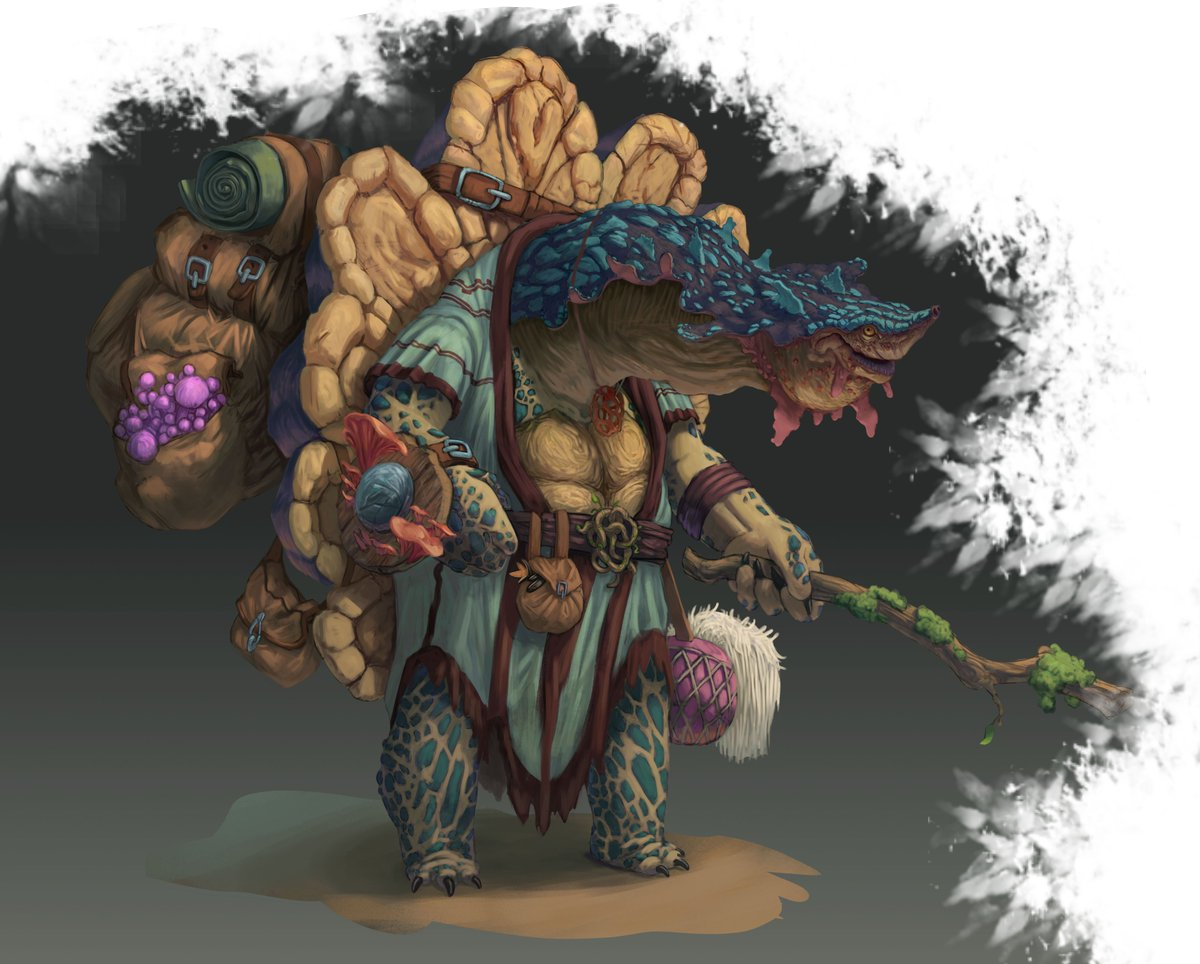
\includegraphics[width=0.52\pdfpagewidth]{05background/img/20tortle_mycolomancer}};
        \end{tikzpicture}

        \newpage

        \subsubsection{Unsettling Words} \label{feat::unsettlingwords}
            You can spin words laced with malice that unsettle a creature and cause it to doubt itself.
            Using one action, you can choose one creature you can see within 12 meters of you.
            Roll a d6.
            The creature must subtract the number rolled from the next saving throw it makes before the start of your next turn.
            A creature can only be affected by this once per round.

            You can use this feature a number of times equal to your Charisma modifier (a minimum of once).
            You regain any expended uses when you finish a short rest.

            You can take this feat additional times to improve the die.
            On a second time it becomes a d8, on a third a d10, and on a fourth a d12.
            \paragraph{Requirements} Merchant background.
\subsection*{Noble} \label{ssec::noble}
    You understand wealth, power, and privilege.
    You carry a noble title, and your family owns land, collects taxes, and wields significant political influence.
    You might be a pampered aristocrat unfamiliar with work or discomfort, a former merchant just elevated to the nobility, or a champion who gained status via knighthood.
    Or you could be an honest, hard-working landowner who cares deeply about the people who live and work on your land, keenly aware of your responsibility to them.

    \subparagraph{Competences} History, plus your choice of two from among Deception, Persuasion, Religion, or a language of your choice.

    \subparagraph{Equipment} A set of fine clothes, and signet ring with your family's sigil, and a purse containing 25 agnomas.

    \subsubsection{Position of Priviledge}
        Thanks to your noble birth, people are inclined to think the best of you.
        You are welcome in high society, and people assume you have the right to be wherever you are.
        The common folk make every effort to accommodate you and avoid your displeasure, and other people of high birth treat you as a member of the same social sphere.
        You can secure an audience with a local noble if you need to.

        You can exert leverage over one or more individuals below you in the social hierarchy and demand their help as needs warrant.
        For example, you can have a message carried across a neighborhood, procure a short carriage ride without paying, or have others clean up a bloody mess you left in an alley.
        The DM decides if your demands are reasonable and if there are people available and willing to fulfill them.
        As your social status improves, you gain influence over more people, including ones in greater positions of power.

    \subsection*{Noble Feats}
        \begin{DndTable}[width=\linewidth, header=Noble Feats]{ll}
            Noble & \textbf{Courtier} (page \pageref{feat::courtier})                 \\
            Noble & \textbf{Early Training} (page \pageref{feat::earlytraining})      \\
            Noble & \textbf{Kept in Style} (page \pageref{feat::keptinstyle})         \\
            Noble & \textbf{Legalese} (page \pageref{feat::legalese})                 \\
            Noble & \textbf{Promise of Status} (page \pageref{feat::promiseofstatus}) \\
            Noble & \textbf{Retainers} (page \pageref{feat::retainers})
        \end{DndTable}

        \subsubsection{Early Training} \label{feat::earlytraining}
            From an early age, your family procured only the best education for you.
            You learn one Fighting Style (see page \pageref{ssec::fightingstyles}) of your choice.
            If you already have a style, the one you choose must be different.
            \paragraph{Requirements} Noble background.
        \subsubsection{Kept in Style (2 FP)} \label{feat::keptinstyle}
            Your family is known across the realm, and your attitude reflects this.
            Your name and signet are sufficient to cover most of your expenses, since everyone would prefer to be in your family's good graces.

            This advantage enables you and your companions to receive most services for free, as long as the cost doesn't rise above 10 agnomas.
            For services up to 50 agnomas, roll a Charisma (Persuasion) check contested by the target's Wisdom (Insight).
            On a success, you can enjoy the service for free.

            At the DM discretion, this feat may be used for more expensive or rarer services, perhaps with disadvantage on the roll or by promising a reward to the service provider.
            \paragraph{Requirements} Noble background.
        \subsubsection{Legalese} \label{feat::legalese}
            Your experience with your local legal system has given you a firm knowledge of the ins and outs of that system.
            Even when the law is not on your side, you can use complex terms like ``ex injuria jus non oritur'' and ``cogitationis poenam nemo patitur'' to frighten people into thinking you know what you're talking about.
            With common folks who don't know any better, you might be able to intimidate or deceive to get favors or special treatment.
            \paragraph{Requirements} Noble or Scholar background.
        \subsubsection{Promise of Status} \label{feat::promiseofstatus}
            Using two actions, you shout your family name to inspire fear from your enemies.
            Each creature that can hear and understand you within 6 meters of you must succeed on a DC 12 Charisma saving throw.
            On a failure, the creature is frightened of you until the end of your next turn.
            At the DM's discretion, a creature might alternatively cease fighting altogether or even join your cause, expecting retribution from your family afterwards.

            You can use this ability a number of times per short rest equal to your Charisma modifier (Minimum of one).

            You can learn this feat a total of three times, increasing the DC to 15 the second time and to 18 the third.
            \paragraph{Requirements} Noble background
        \subsubsection{Retainers} \label{feat::retainers}
            You gain the service of three retainers loyal to your family.
            These retainers can be attendants or messengers, and one might be a majordomo.
            One of your retainers can serve as your squire, aiding you in exchange for training on their own path to knighthood.
            Another retainer might be a groom to care for your horse or a servant who polishes your armor and helps you put it on.

            Your retainers can perform mundane tasks for you, but they do not fight for you, follow you into obviously dangerous areas (such as dungeons).
            Your retainers will leave if they are frequently endangered or abused, and it will take your family 1d6 weeks to send you a new group.
            \paragraph{Requirements} Noble background.
\subsection*{Sailor} \label{ssec::sailor}
    You sailed on a seagoing vessel for years.
    In that time, you faced down mighty storms, monsters of the deep, and those who wanted to sink your craft to the bottomless depths.
    Your first love is the distant line of the horizon.

    Discuss the nature of the ship you previously sailed with your Dungeon Master.
    Was it a merchant ship, a naval vessel, a ship of discovery, or a pirate ship?
    How famous (or infamous) is it?
    Is it widely traveled?
    Is it still sailing, or is it missing and presumed lost with all hands?
    What were your duties on board?

    \subparagraph{Competences} Water vehicles, plus your choice of two from among Perception, Survival, Navigator's Tools, or Carpenter's Tools.

    \subparagraph{Equipment} A belaying pin, 50 feet of silk rope, a lucky charm, and a set of common clothes.

    \subsubsection{Ship's Passage}
        When you need to, you can secure free passage on a sailing ship for yourself and your companions.
        You might sail on the ship you served on, or another ship you have good relations with (perhaps one captained by a former crewmate).
        Because you're calling in a favor, you can't be certain of a schedule or route that will meet your every need.
        Your Dungeon Master will determine how long it takes to get where you need to go.
        In return for your free passage, you and your companions are expected to assist the crew during the voyage.

    \subsection*{Sailor Feats}
        \begin{DndTable}[width=\linewidth, header=Sailor Feats]{ll}
            Sailor & \textbf{Drunken Resilience} (page \pageref{feat::drunkenresilience}) \\
            Sailor & \textbf{Expert Stirrer} (page \pageref{feat::expertstirrer})         \\
            Sailor & \textbf{Harvest the Water} (page \pageref{feat::harvestthewater})    \\
            Sailor & \textbf{I'll Patch It} (page \pageref{feat::illpatchit})             \\
            Sailor & \textbf{Sailor's Balance} (page \pageref{feat::sailorsbalance})      \\
            Sailor & \textbf{Wisdom of the Wilds} (page \pageref{feat::wisdomofthewilds})
        \end{DndTable}

        \subsubsection{Drunken Resilience (2 FP)} \label{feat::drunkenresilience}
            You can drink enough alcohol to knock an elephant.
            You have advantage on saving throws against poison, and you have resistance against poison damage.
            \paragraph{Requirements} Sailor background.
        \subsubsection{Expert Stirrer} \label{feat::expertstirrer}
            Years of arguing and interacting at seas have made your insults extraordinarily effective.
            As an action, you can hurl a terrible insult to a creature within 12 meters of you who can hear you and understand your language.
            The creature must roll a DC 12 Wisdom saving throw.
            On a failure, the creature has disadvantage on attack rolls against targets other than you and can't make opportunity attacks against targets other than you.
            This effect lasts for 1 minute, until one of your companions attacks the target or affects it with a spell, or until you and the target are more than 12 meters apart.

            You can use this ability a number of times per short rest equal to your Charisma modifier (Minimum of one).

            You can learn this feat a total of three times, increasing the DC to 15 the second time and to 18 the third.
            \paragraph{Requirements} Sailor background.
        \subsubsection{Harvest the Water} \label{feat::harvestthewater}
            You gain advantage on ability checks made using fishing tackle.
            If you have access to a body of water that sustains marine life, you can maintain a moderate lifestyle while working as a fisher, and you can catch enough food to feed yourself and up to ten other people each day.
            \paragraph{Requirements} Sailor background.
        \subsubsection{I'll Patch It!} \label{feat::illpatchit}
            Provided you have carpenter's tools and wood, you can perform repairs on a water vehicle.
            You don't need to be competent with carpenter's tools to gain this feat.
            When you use this ability, you restore a number of hit points to the hull of a water vehicle equal to twice your level.
            A vehicle cannot be patched by you in this way again until you finish a short rest.
            \paragraph{Requirements} Sailor background.
        \subsubsection{Sailor's Balance} \label{feat::sailorsbalance}
            Used to the ever-present swing of a ship, you have advantage on any ability checks and saving throws made to avoid being moved or being knocked prone.
            \paragraph{Requirements} Sailor background.
        \subsubsection{Wisdom of the Wilds} \label{feat::wisdomofthewilds}
            Your extended travels have given you a special appreciation for the stillness of the world.
            After finishing a short rest, you gain temporary hit points equal to your level + your Wisdom modifier, and you have advantage on the first ability check you make during the day.
            \paragraph{Requirements} Sailor or Outlander background.
\subsection*{Scholar} \label{ssec::scholar}
    Sages, scholars, students, and scientists are all passionate about one or many fields of study.
    You are defined by your extensive studies, and your characteristics reflect this life of study.
    Devoted to scholarly pursuits, you value knowledge highly --- sometimes in its own right, sometimes as a means toward other ideals.

    \subparagraph{Competences} Investigation, plus your choice of two from among Arcana, History, Medicine, or one language.

    \subparagraph{Equipment} A bottle of black ink, a quill, a small knife, a letter from a dead colleague posing a question you have not yet been able to answer, and a set of common clothes.

    \subsubsection{Researcher} \label{feat::researcher}
        When you attempt to learn or recall a piece of lore, if you do not know that information, you often know where and from whom you can obtain it.
        Usually, this information comes from a library, scriptorium, university, or a sage or other learned person or creature.
        Your DM might rule that the knowledge you seek is secreted away in an almost inaccessible place, or that it simply cannot be found.

    \subsection*{Scholar Feats}
        \begin{DndTable}[width=\linewidth, header=Scholar Feats]{ll}
            Scholar & \textbf{Adept Linguist} (page \pageref{feat::adeptlinguist})             \\
            Scholar & \textbf{Flash of Genius} (page \pageref{feat::flashofgenius})            \\
            Scholar & \textbf{Historical Knowledge} (page \pageref{feat::historicalknowledge}) \\
            Scholar & \textbf{Legalese} (page \pageref{feat::legalese})                        \\
            Scholar & \textbf{Metamagic Adept} (page \pageref{feat::metamagicadept})           \\
            Scholar & \textbf{Skill Versatility} (page \pageref{feat::skillversatility})
        \end{DndTable}

        \subsubsection{Adept Linguist} \label{feat::adeptlinguist}
            You can communicate with people who don't speak any language you know.
            You must observe the people interacting with one another for at least 1 day, after which you learn a handful of important words, expressions, and gestures --- enough to communicate on a rudimentary level.
            \paragraph{Requirements} Scholar background.
        \subsubsection{Historical Knowledge} \label{feat::historicalknowledge}
            When you enter a ruin or dungeon, you can correctly ascertain its original purpose and determine its builders, whether those were gats, oths, ets, thri-kreen, or some other known kin.
            In addition, you can determine the monetary value of art objects more than a century old.
            \paragraph{Requirements} Scholar background.
        \subsubsection{Metamagic Adept} \label{feat::metamagicadept}
            By understanding the relation between a variety of doctrines, you've learned how to exert your will on your spells to alter how they function.
            You learn one spellcasting feat that requires an ability score different than your chosen spellcasting ability score.
            The FP cost of the feat for you is increased by 1.

            You can take this feat 3 times, learning a new feat the second and third time.
            \paragraph{Requirements} Scholar background and Spellcasting feat.
        \subsubsection{Skill Versatility (2 FP)} \label{feat::skillversatility}
            Your life of studies has given you the capacity to quickly learn new subjects.
            You gain two proficiency levels on a skill of your choice.
            This skill must be related to Intelligence or Wisdom.

            After a long rest, you can chance this proficiency to another skill, also related to Intelligence or Wisdom.
            \paragraph{Requirements} Scholar background.
\subsection*{Soldier} \label{ssec::soldier}
    You trained as a youth, studied the use of weapons and armor, learned basic survival techniques. %, including how to stay alive on the battlefield.
    You might have been part of a standing army or a mercenary company, or perhaps a member of a local militia who rose to prominence during a recent war.

    % \newpage

    When you choose this background, work with your DM to determine which organization you were a part of, how far through its ranks you progressed, and what kind of experiences you had during your career.
    Was it a standing army, a town guard, or a village militia?
    Or it might have been a noble's order of knights, a merchant's private army, or a mercenary company.

    \subparagraph{Competences} Competence with a weapon type of your choice, plus your choice of two from among Athletics, Intimidation, an armor type of your choice, or land vehicles.

    \subparagraph{Equipment} An insignia of rank, a trophy taken from a fallen enemy, and a set of common clothes.

    \subsubsection{Military Rank}
        You have a military rank from your career as a soldier.
        Soldiers loyal to your former military organization still recognize your authority and influence, and they defer to you if they are of a lower rank.
        You can invoke your rank to exert influence over other soldiers and requisition simple equipment or horses for temporary use.
        You can also usually gain access to friendly military encampments and fortresses where your rank is recognized.

    \subsection*{Soldier Feats}
        \begin{DndTable}[width=\linewidth, header=Soldier Feats]{ll}
            Soldier & \textbf{Inspiring Leader} (page \pageref{feat::inspiringleader})      \\
            Soldier & \textbf{Know your Enemy} (page \pageref{feat::knowyourenemy})         \\
            Soldier & \textbf{Martial Adept} (page \pageref{feat::martialadept})            \\
            Soldier & \textbf{Official Inquirt} (page \pageref{feat::officialinquiry})      \\
            Soldier & \textbf{Soldier's Fortitude} (page \pageref{feat::soldiersfortitude}) \\
            Soldier & \textbf{Steady} (page \pageref{feat::steady})
        \end{DndTable}

        \subsubsection{Know your Enemy} \label{feat::knowyourenemy}
            If you spend at least 1 minute observing or interacting with another creature outside combat, you can learn certain information about its capabilities compared to your own.
            The DM tells you if the creature is your equal, superior, or inferior in regard to two of the following characteristics of your choice:
            \begin{itemize}
                \item Strength score
                \item Dexterity score
                \item Constitution score
                \item Armor Class
                \item Current hit points
                \item Total levels
            \end{itemize}
            \paragraph{Requirements} Soldier background.
        \subsubsection{Martial Adept} \label{feat::martialadept}
            You have martial training that allows you to learn advanced combat techniques.
            You learn one feat of your choice from any fighting style that you don't already have.
            The FP cost of the feat for you is increased by 1.

            You can take this feat 3 times, learning a new feat the second and third time.
            \paragraph{Requirements} Soldier background.
        \subsubsection{Official Inquiry} \label{feat::officialinquiry}
            You're experienced at gaining access to people and places to get the information you need.
            Through a combination of fast-talking, determination, and official-looking documentation, you can gain access to a place or an individual related to a something you're investigating.
            Those who aren't involved in your investigation avoid impeding you or pass along your requests.
            \paragraph{Requirements} Soldier background.
        \subsubsection{Soldier's Fortitude (2 FP)} \label{feat::soldiersfortitude}
            Whenever you take the Dodge action in combat, you can spend one hit die to heal yourself.
            Roll the die, add your Constitution modifier, and regain a number of hit points equal to the total (minimum of 1).
            \paragraph{Requirements} Soldier background.
        \subsubsection{Steady} \label{feat::steady}
            You can move twice the normal amount of time (up to 16 hours) each day before being subject to the effect of a forced march (see ``Travel Pace'' in chapter 8 of the Player's Handbook).
            \paragraph{Requirements} Outlander or Soldier background.
\subsection*{Outlander} \label{ssec::outlander}
    Either by choice or by birthright, you have spent much of your life in the wilds, far from the comforts of civilization.
    You've witnessed the migration of herds larger than forests, survived weather more extreme than any city-dweller could comprehend, and enjoyed the solitude of being the only thinking creature for miles in any direction.
    The wilds are in your blood, whether you were a nomad, an explorer, a recluse, a hunter-gatherer, or a hermit.
    Even in places where you don't know the specific features of the terrain, you know the ways of the wild.

    \subparagraph{Competences} Survival, plus your choice of two from among Animal Handling, Athletics, Nature, or a musical instrument.

    \subparagraph{Equipment} A staff, a hunting trap, a trophy from nature, and a set of traveler's clothes.

    \subsubsection{Wanderer}
        % You have an excellent memory for maps and geography, and you can always recall the general layout of terrain, settlements, and other features around you.
        You can always recall the general layout of terrain, settlements, and other features around you.
        In addition, you can find food and fresh water for yourself and up to five other people each day, provided that the land offers berries, small game, water, and so forth.

    \subsection*{Outlander Feats}
        \begin{DndTable}[width=\linewidth, header=Outlander Feats]{ll}
            Outlander & \textbf{All Eyes on You} (page \pageref{feat::alleyesonyou})         \\
            Outlander & \textbf{Land's Stride} (page \pageref{feat::landsstride})            \\
            Outlander & \textbf{Nature's Heritage} (page \pageref{feat::naturesheritage})    \\
            Outlander & \textbf{Roving} (page \pageref{feat::roving})                        \\
            Outlander & \textbf{Steady} (page \pageref{feat::steady})                        \\
            Outlander & \textbf{Wisdom of the Wilds} (page \pageref{feat::wisdomofthewilds})
        \end{DndTable}

        \subsubsection{All Eyes on You} \label{feat::alleyesonyou}
        Your accent, mannerisms, figures of speech, and perhaps even your appearance all mark you as foreign.
        You gain the friendly interest of scholars and others intrigued by far-removed lands, to say nothing of everyday folk who are eager to hear stories of your origin.

        You can parley this attention into access to people and places you might not otherwise have, for you and your traveling companions.
        Noble lords, scholars, and merchant princes, to name a few, might be interested in hearing about your homeland.
        \paragraph{Requirements} Outlander background.
        \subsubsection{Land's Stride (2 FP)} \label{feat::landsstride}
        Moving through difficult terrain costs you no extra movement.
        You can also pass through plants without being slowed by them and without taking damage from them if they have thorns, spines, or a similar hazard.

        In addition, you have advantage on saving throws against plants that are magically created or manipulated to impede movement, such those created by the entangle spell.
        \paragraph{Requirements} Outlander background.
        \subsubsection{Nature's Heritage} \label{feat::naturesheritage}
        You are familiar enough with any wilderness area that you can find twice as much food and water as you normally would when you forage.
        \paragraph{Requirements} Outlander background.
        \subsubsection{Roving} \label{feat::roving}
        A deft explorer, your movement is unimpeded by water or mountain.
        You can take this feat three times, gaining different abilities each time:
        \begin{itemize}
            \item The first time, you gain a swimming speed equal to your walking speed.
            \item The second time, you can a climbing speed equal to your walking speed.
            \item The third time, your walking speed is increased by 1 meter.
        \end{itemize}
        After gaining the first or second abilities from this feat, Any effect that increases your movement speed also increases your swimming and climbing speed by the same amount.
        \paragraph{Requirements} Outlander background.

\newpage

% NOTE. Unused background feats.
% \subsubsection{Inheritance} \label{feat::inheritance}
%     Choose or randomly determine your inheritance from the possibilities in the table below.
%     Work with your Dungeon Master to come up with details: Why is your inheritance so important, and what is its full story?
%     You might prefer for the DM to invent these details as part of the game, allowing you to learn more about your inheritance as your character does.
%
%     The Dungeon Master is free to use your inheritance as a story hook, sending you on quests to learn more about its history or true nature, or confronting you with foes who want to claim it for themselves or prevent you from learning what you seek.
%     The DM also determines the properties of your inheritance and how they figure into the item's history and importance.
%     For instance, the object might be a minor magic item, or one that begins with a modest ability and increases in potency with the passage of time.
%     Or, the true nature of your inheritance might not be apparent at first and is revealed only when certain conditions are met.
%
%     You can decide whether or when to tell your companions about your inheritance.
%     Rather than attracting attention to yourself, you might want to keep your inheritance a secret until you learn more about what it means to you and what it can do for you.
%
%     \begin{DndTable}[width=\linewidth, header=Inheritance]{cX}
%         \textbf{d8} & \textbf{Object or item}                                  \\
%         1   & A document such as a map, a letter, or a journal                 \\
%         2-3 & a trinket (see "Trinkets" in chapter 5 of the Player's Handbook) \\
%         4   & an article of clothing                                           \\
%         5   & a piece of jewelry                                               \\
%         6   & an arcane book or formulary                                      \\
%         7   & a written story, song, poem, or secret                           \\
%         8   & a tattoo or other body marking
%     \end{DndTable}
%     \paragraph{Requirements} Noble background.
% J
% \subsubsection{Library Access} \label{feat::libraryaccess}
    %     You are a well-known scholar (or good enough at pretending to be one), and have free and easy access to the majority of libraries.
    %     This doesn't give you access to repositories of lore that are too valuable or secret to permit anyone immediate access.
    %
    %     Additionally, you are likely to gain preferential treatment at libraries and universities accross Yuadrem, as professional courtesy to a fellow scholar.
    %     \paragraph{Requirements} Scholar background.
    % M
% \subsubsection{Mercenary Life} \label{feat::mercenarylife}
%     You know local mercenaries as only someone who has worked with them can.
%     You are able to identify mercenary companies by their emblems, and you know a little about any such company, including who has hired them recently.
%     You can find the taverns and festhalls where mercenaries abide in any area, as long as you speak the language.
%     You can find mercenary work between adventures sufficient to maintain a comfortable lifestyle.
%     \paragraph{Requirements} Soldier background.
% \subsubsection{Watcher's Eye} \label{feat::watcherseye}
%     Your experience in enforcing the law, and dealing with lawbreakers, gives you a feel for local laws and criminals.
%     You can easily find the local outpost of the watch or a similar organization, and just as easily pick out the dens of criminal activity in a community, although you're more likely to be welcome in the former locations rather than the latter.
%     \paragraph{Requirements} Soldier background.
